% Options for packages loaded elsewhere
\PassOptionsToPackage{unicode}{hyperref}
\PassOptionsToPackage{hyphens}{url}
\PassOptionsToPackage{dvipsnames,svgnames,x11names}{xcolor}
%
\documentclass[
  letterpaper,
  DIV=11,
  numbers=noendperiod]{scrartcl}

\usepackage{amsmath,amssymb}
\usepackage{iftex}
\ifPDFTeX
  \usepackage[T1]{fontenc}
  \usepackage[utf8]{inputenc}
  \usepackage{textcomp} % provide euro and other symbols
\else % if luatex or xetex
  \usepackage{unicode-math}
  \defaultfontfeatures{Scale=MatchLowercase}
  \defaultfontfeatures[\rmfamily]{Ligatures=TeX,Scale=1}
\fi
\usepackage{lmodern}
\ifPDFTeX\else  
    % xetex/luatex font selection
\fi
% Use upquote if available, for straight quotes in verbatim environments
\IfFileExists{upquote.sty}{\usepackage{upquote}}{}
\IfFileExists{microtype.sty}{% use microtype if available
  \usepackage[]{microtype}
  \UseMicrotypeSet[protrusion]{basicmath} % disable protrusion for tt fonts
}{}
\makeatletter
\@ifundefined{KOMAClassName}{% if non-KOMA class
  \IfFileExists{parskip.sty}{%
    \usepackage{parskip}
  }{% else
    \setlength{\parindent}{0pt}
    \setlength{\parskip}{6pt plus 2pt minus 1pt}}
}{% if KOMA class
  \KOMAoptions{parskip=half}}
\makeatother
\usepackage{xcolor}
\setlength{\emergencystretch}{3em} % prevent overfull lines
\setcounter{secnumdepth}{-\maxdimen} % remove section numbering
% Make \paragraph and \subparagraph free-standing
\ifx\paragraph\undefined\else
  \let\oldparagraph\paragraph
  \renewcommand{\paragraph}[1]{\oldparagraph{#1}\mbox{}}
\fi
\ifx\subparagraph\undefined\else
  \let\oldsubparagraph\subparagraph
  \renewcommand{\subparagraph}[1]{\oldsubparagraph{#1}\mbox{}}
\fi

\usepackage{color}
\usepackage{fancyvrb}
\newcommand{\VerbBar}{|}
\newcommand{\VERB}{\Verb[commandchars=\\\{\}]}
\DefineVerbatimEnvironment{Highlighting}{Verbatim}{commandchars=\\\{\}}
% Add ',fontsize=\small' for more characters per line
\usepackage{framed}
\definecolor{shadecolor}{RGB}{241,243,245}
\newenvironment{Shaded}{\begin{snugshade}}{\end{snugshade}}
\newcommand{\AlertTok}[1]{\textcolor[rgb]{0.68,0.00,0.00}{#1}}
\newcommand{\AnnotationTok}[1]{\textcolor[rgb]{0.37,0.37,0.37}{#1}}
\newcommand{\AttributeTok}[1]{\textcolor[rgb]{0.40,0.45,0.13}{#1}}
\newcommand{\BaseNTok}[1]{\textcolor[rgb]{0.68,0.00,0.00}{#1}}
\newcommand{\BuiltInTok}[1]{\textcolor[rgb]{0.00,0.23,0.31}{#1}}
\newcommand{\CharTok}[1]{\textcolor[rgb]{0.13,0.47,0.30}{#1}}
\newcommand{\CommentTok}[1]{\textcolor[rgb]{0.37,0.37,0.37}{#1}}
\newcommand{\CommentVarTok}[1]{\textcolor[rgb]{0.37,0.37,0.37}{\textit{#1}}}
\newcommand{\ConstantTok}[1]{\textcolor[rgb]{0.56,0.35,0.01}{#1}}
\newcommand{\ControlFlowTok}[1]{\textcolor[rgb]{0.00,0.23,0.31}{#1}}
\newcommand{\DataTypeTok}[1]{\textcolor[rgb]{0.68,0.00,0.00}{#1}}
\newcommand{\DecValTok}[1]{\textcolor[rgb]{0.68,0.00,0.00}{#1}}
\newcommand{\DocumentationTok}[1]{\textcolor[rgb]{0.37,0.37,0.37}{\textit{#1}}}
\newcommand{\ErrorTok}[1]{\textcolor[rgb]{0.68,0.00,0.00}{#1}}
\newcommand{\ExtensionTok}[1]{\textcolor[rgb]{0.00,0.23,0.31}{#1}}
\newcommand{\FloatTok}[1]{\textcolor[rgb]{0.68,0.00,0.00}{#1}}
\newcommand{\FunctionTok}[1]{\textcolor[rgb]{0.28,0.35,0.67}{#1}}
\newcommand{\ImportTok}[1]{\textcolor[rgb]{0.00,0.46,0.62}{#1}}
\newcommand{\InformationTok}[1]{\textcolor[rgb]{0.37,0.37,0.37}{#1}}
\newcommand{\KeywordTok}[1]{\textcolor[rgb]{0.00,0.23,0.31}{#1}}
\newcommand{\NormalTok}[1]{\textcolor[rgb]{0.00,0.23,0.31}{#1}}
\newcommand{\OperatorTok}[1]{\textcolor[rgb]{0.37,0.37,0.37}{#1}}
\newcommand{\OtherTok}[1]{\textcolor[rgb]{0.00,0.23,0.31}{#1}}
\newcommand{\PreprocessorTok}[1]{\textcolor[rgb]{0.68,0.00,0.00}{#1}}
\newcommand{\RegionMarkerTok}[1]{\textcolor[rgb]{0.00,0.23,0.31}{#1}}
\newcommand{\SpecialCharTok}[1]{\textcolor[rgb]{0.37,0.37,0.37}{#1}}
\newcommand{\SpecialStringTok}[1]{\textcolor[rgb]{0.13,0.47,0.30}{#1}}
\newcommand{\StringTok}[1]{\textcolor[rgb]{0.13,0.47,0.30}{#1}}
\newcommand{\VariableTok}[1]{\textcolor[rgb]{0.07,0.07,0.07}{#1}}
\newcommand{\VerbatimStringTok}[1]{\textcolor[rgb]{0.13,0.47,0.30}{#1}}
\newcommand{\WarningTok}[1]{\textcolor[rgb]{0.37,0.37,0.37}{\textit{#1}}}

\providecommand{\tightlist}{%
  \setlength{\itemsep}{0pt}\setlength{\parskip}{0pt}}\usepackage{longtable,booktabs,array}
\usepackage{calc} % for calculating minipage widths
% Correct order of tables after \paragraph or \subparagraph
\usepackage{etoolbox}
\makeatletter
\patchcmd\longtable{\par}{\if@noskipsec\mbox{}\fi\par}{}{}
\makeatother
% Allow footnotes in longtable head/foot
\IfFileExists{footnotehyper.sty}{\usepackage{footnotehyper}}{\usepackage{footnote}}
\makesavenoteenv{longtable}
\usepackage{graphicx}
\makeatletter
\def\maxwidth{\ifdim\Gin@nat@width>\linewidth\linewidth\else\Gin@nat@width\fi}
\def\maxheight{\ifdim\Gin@nat@height>\textheight\textheight\else\Gin@nat@height\fi}
\makeatother
% Scale images if necessary, so that they will not overflow the page
% margins by default, and it is still possible to overwrite the defaults
% using explicit options in \includegraphics[width, height, ...]{}
\setkeys{Gin}{width=\maxwidth,height=\maxheight,keepaspectratio}
% Set default figure placement to htbp
\makeatletter
\def\fps@figure{htbp}
\makeatother

\KOMAoption{captions}{tableheading}
\makeatletter
\makeatother
\makeatletter
\makeatother
\makeatletter
\@ifpackageloaded{caption}{}{\usepackage{caption}}
\AtBeginDocument{%
\ifdefined\contentsname
  \renewcommand*\contentsname{Table of contents}
\else
  \newcommand\contentsname{Table of contents}
\fi
\ifdefined\listfigurename
  \renewcommand*\listfigurename{List of Figures}
\else
  \newcommand\listfigurename{List of Figures}
\fi
\ifdefined\listtablename
  \renewcommand*\listtablename{List of Tables}
\else
  \newcommand\listtablename{List of Tables}
\fi
\ifdefined\figurename
  \renewcommand*\figurename{Figure}
\else
  \newcommand\figurename{Figure}
\fi
\ifdefined\tablename
  \renewcommand*\tablename{Table}
\else
  \newcommand\tablename{Table}
\fi
}
\@ifpackageloaded{float}{}{\usepackage{float}}
\floatstyle{ruled}
\@ifundefined{c@chapter}{\newfloat{codelisting}{h}{lop}}{\newfloat{codelisting}{h}{lop}[chapter]}
\floatname{codelisting}{Listing}
\newcommand*\listoflistings{\listof{codelisting}{List of Listings}}
\makeatother
\makeatletter
\@ifpackageloaded{caption}{}{\usepackage{caption}}
\@ifpackageloaded{subcaption}{}{\usepackage{subcaption}}
\makeatother
\makeatletter
\@ifpackageloaded{tcolorbox}{}{\usepackage[skins,breakable]{tcolorbox}}
\makeatother
\makeatletter
\@ifundefined{shadecolor}{\definecolor{shadecolor}{rgb}{.97, .97, .97}}
\makeatother
\makeatletter
\makeatother
\makeatletter
\makeatother
\ifLuaTeX
  \usepackage{selnolig}  % disable illegal ligatures
\fi
\IfFileExists{bookmark.sty}{\usepackage{bookmark}}{\usepackage{hyperref}}
\IfFileExists{xurl.sty}{\usepackage{xurl}}{} % add URL line breaks if available
\urlstyle{same} % disable monospaced font for URLs
\hypersetup{
  pdftitle={BuseBakis Homework 1},
  pdfauthor={Buse Bakış},
  colorlinks=true,
  linkcolor={blue},
  filecolor={Maroon},
  citecolor={Blue},
  urlcolor={Blue},
  pdfcreator={LaTeX via pandoc}}

\title{BuseBakis Homework 1}
\author{Buse Bakış}
\date{}

\begin{document}
\maketitle
\ifdefined\Shaded\renewenvironment{Shaded}{\begin{tcolorbox}[breakable, sharp corners, borderline west={3pt}{0pt}{shadecolor}, interior hidden, enhanced, boxrule=0pt, frame hidden]}{\end{tcolorbox}}\fi

\hypertarget{project-start}{%
\section{Project start}\label{project-start}}

In this chapter, we are going to work together on a very simple project.
This project will stay with us until the end of the book. As we will go
deeper into the book together, you will rewrite that project by
implementing the techniques I will teach you. By the end of the book you
will have built a reproducible analytical pipeline. To get things going,
we are going to keep it simple; our goal here is to get an analysis
done, that's it. We won't focus on reproducibility. We are going to
download some data, and analyse it, that's it.

\hypertarget{housing-in-luxembourg}{%
\subsection{Housing in Luxembourg}\label{housing-in-luxembourg}}

We are going to download data about house prices in Luxembourg.
Luxembourg is a little Western European country the author hails from
that looks like a shoe and is about the size of .98 Rhode Islands. Did
you know that Luxembourg is a constitutional monarchy, and not a kingdom
like Belgium, but a Grand-Duchy, and actually the last Grand-Duchy in
the World? Also, what you should know to understand what we will be
doing is that the country of Luxembourg is divided into Cantons, and
each Cantons into Communes. If Luxembourg was the USA, Cantons would be
States and Communes would be Counties (or Parishes or Boroughs). What's
confusing is that ``Luxembourg'' is also the name of a Canton, and of a
Commune, which also has the status of a city and is the capital of the
country. So Luxembourg the country, is divided into Cantons, one of
which is called Luxembourg as well, cantons are divided into communes,
and inside the canton of Luxembourg, there's the commune of Luxembourg
which is also the city of Luxembourg, sometimes called Luxembourg City,
which is the capital of the country.

\begin{figure}

{\centering 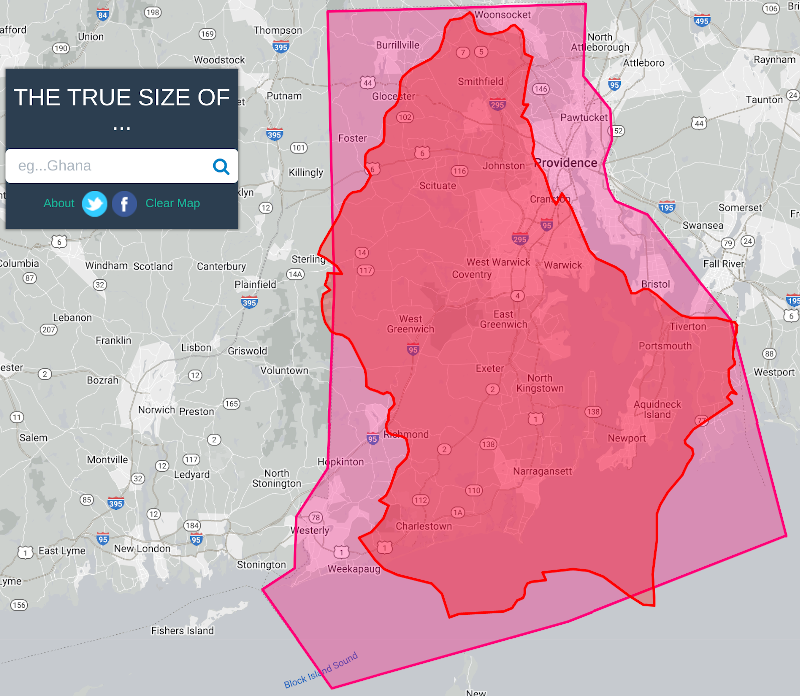
\includegraphics[width=3.125in,height=\textheight]{images/lux_rhode_island.png}

}

\caption{Luxembourg is about as big as the US State of Rhode Island.}

\end{figure}

What you should also know is that the population is about 645,000 as of
writing (January 2023), half of which are foreigners. Around 400,000
persons work in Luxembourg, of which half do not live in Luxembourg; so
every morning from Monday to Friday, 200,000 people enter the country to
work and then leave in the evening to go back to either Belgium, France
or Germany, the neighbouring countries. As you can imagine, this puts
enormous pressure on the transportation system and on the roads, but
also on the housing market; everyone wants to live in Luxembourg to
avoid the horrible daily commute, and everyone wants to live either in
the capital city, or in the second largest urban area in the south, in a
city called Esch-sur-Alzette.

The plot below shows the value of the House Price Index over time for
Luxembourg and the European Union:

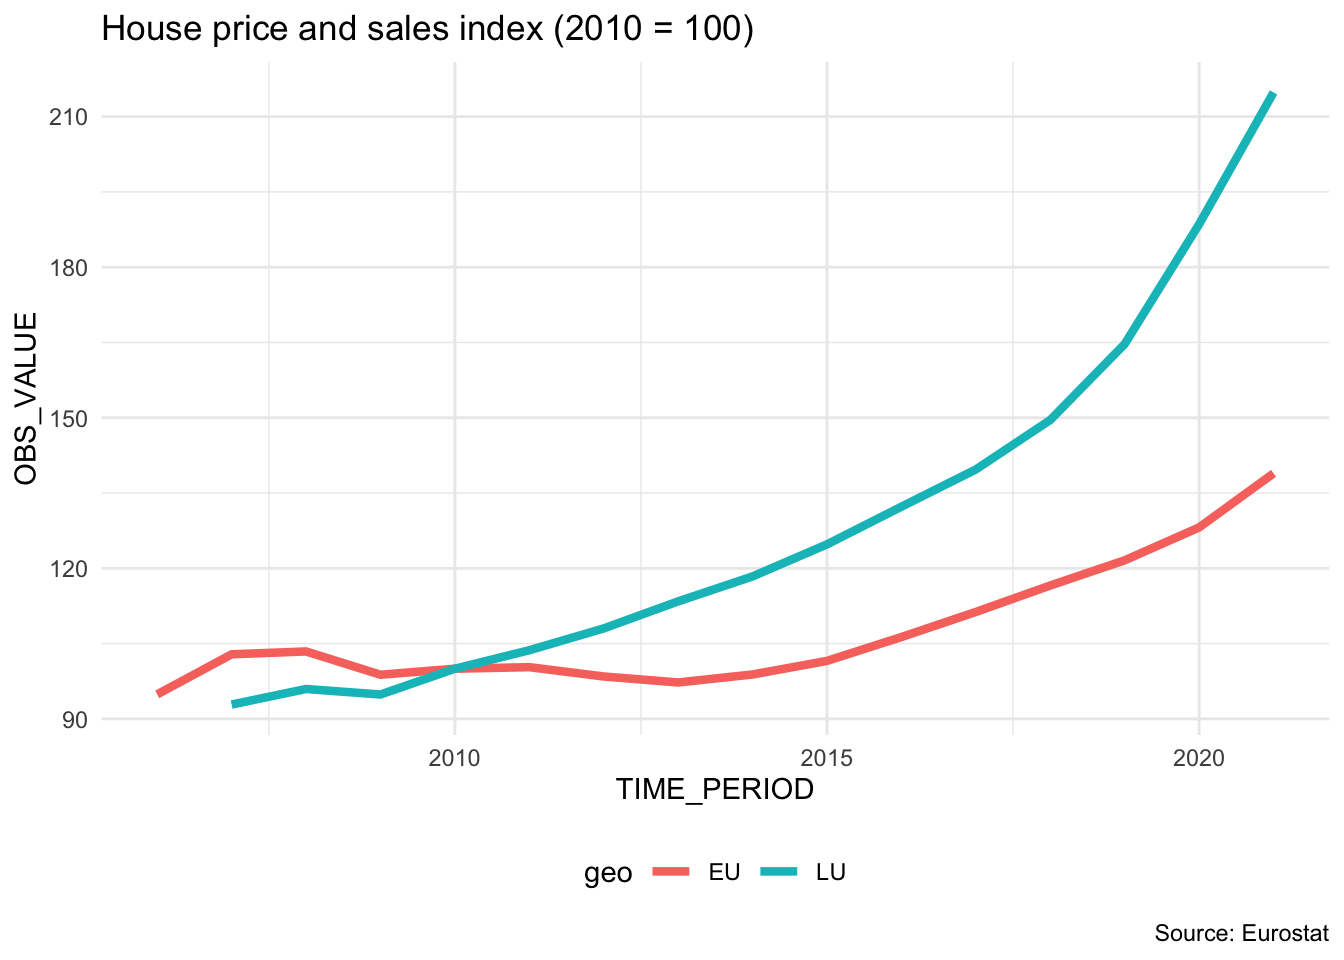
\includegraphics{busebakis_hw1_files/figure-pdf/unnamed-chunk-2-1.pdf}

If you want to download the data, click
\href{https://github.com/b-rodrigues/rap4all/raw/master/datasets/prc_hpi_a__custom_4705395_page_linear.csv.gz}{here}\footnote{https://is.gd/AET0ir}.

Let us paste the definition of the HPI in here (taken from the HPI's
\href{https://archive.is/OrQwA}{metadata}\footnote{https://archive.is/OrQwA,
  archived link for posterity.} page):

\emph{The House Price Index (HPI) measures inflation in the residential
property market. The HPI captures price changes of all types of
dwellings purchased by households (flats, detached houses, terraced
houses, etc.). Only transacted dwellings are considered, self-build
dwellings are excluded. The land component of the dwelling is included.}

So from the plot, we can see that the price of dwellings more than
doubled between 2010 and 2021; the value of the index is 214.81 in 2021
for Luxembourg, and 138.92 for the European Union as a whole.

There is a lot of heterogeneity though; the capital and the communes
right next to the capital are much more expensive than communes from the
less densely populated north, for example. The south of the country is
also more expensive than the north, but not as much as the capital and
surrounding communes. Not only is price driven by demand, but also by
scarcity; in 2021, 0.5\% of residents owned 50\% of the buildable land
for housing purposes (Source: \emph{Observatoire de l'Habitat, Note 29},
\href{https://archive.org/download/note-29/note-29.pdf}{archived
download link}\footnote{https://archive.org/download/note-29/note-29.pdf}).

Our project will be quite simple; we are going to download some data,
supplied as an Excel file, compiled by the Housing Observatory
(\emph{Observatoire de l'Habitat}, a service from the Ministry of
Housing, which monitors the evolution of prices in the housing market,
among other useful services like the identification of vacant lots). The
advantage of their data when compared to Eurostat's data is that the
data is disaggregated by commune. The disadvantage is that they only
supply nominal prices, and no index (and the data is trapped inside
Excel and not ready for analysis with R). Nominal prices are the prices
that you read on price tags in shops. The problem with nominal prices is
that it is difficult to compare them through time. Ask yourself the
following question: would you prefer to have had 500€ (or USDs) in 2003
or in 2023? You probably would have preferred them in 2003, as you could
purchase a lot more with \$500 then than now. In fact, according to a
random inflation calculator I googled, to match the purchasing power of
\$500 in 2003, you'd need to have \$793 in 2023 (and I'd say that we
find very similar values for €). But it doesn't really matter if that
calculation is 100\% correct: what matters is that the value of money
changes, and comparisons through time are difficult, hence why an index
is quite useful. So we are going to convert these nominal prices to real
prices. Real prices take inflation into account and so allow us to
compare prices through time.

So to summarise; our goal is to:

\begin{itemize}
\tightlist
\item
  Get data trapped inside an Excel file into a neat data frame;
\item
  Convert nominal to real prices using a simple method;
\item
  Make some tables and plots and call it a day (for now).
\end{itemize}

We are going to start in the most basic way possible; we are simply
going to write a script and deal with each step separately.

\newpage

\hypertarget{saving-trapped-data-from-excel}{%
\subsection{Saving trapped data from
Excel}\label{saving-trapped-data-from-excel}}

Getting data from Excel into a tidy data frame can be very tricky. This
is because very often, Excel is used as some kind of dashboard or
presentation tool. So data is made human-readable, in contrast to
machine-readable. Let us quickly discuss this topic as it is essential
to grasp the difference between the two (and in our experience, a lot of
collective pain inflicted to statisticians and researchers could have
been avoided if this concept was more well-known). The picture below
shows an Excel file made for human consumption:

\begin{figure}

{\centering 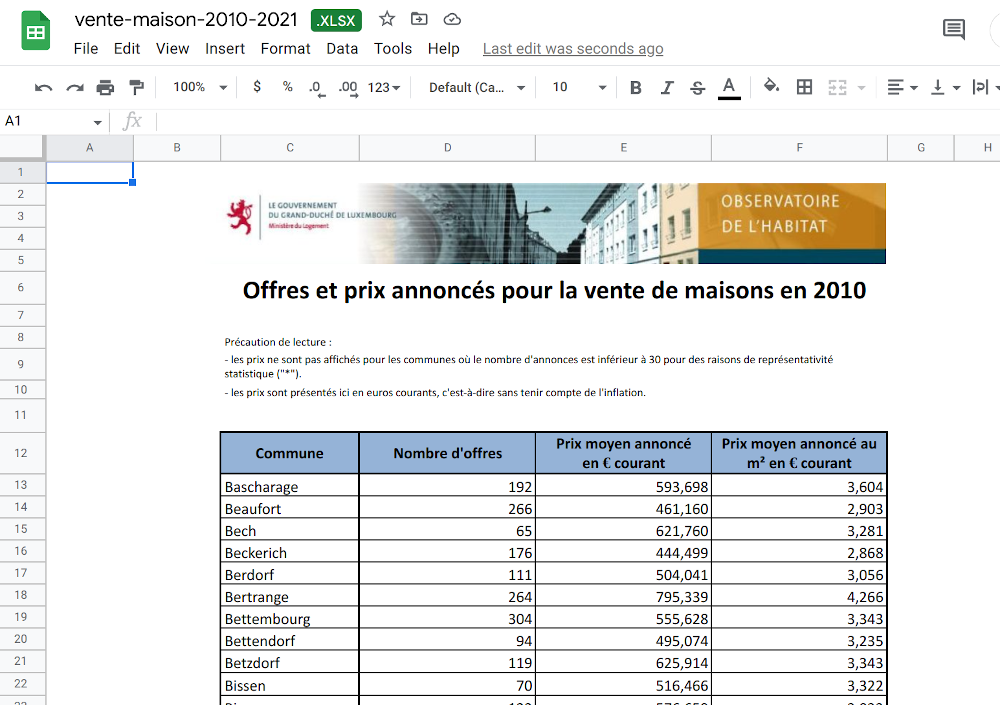
\includegraphics[width=3.33in,height=\textheight]{images/obs_hab_xlsx_overview.png}

}

\caption{An Excel file meant for human eyes.}

\end{figure}

So why is this file not machine-readable? Here are some issues:

\begin{itemize}
\tightlist
\item
  The table does not start in the top-left corner of the spreadsheet,
  which is where most importing tools expect it to be;
\item
  The spreadsheet starts with a header that contains an image and some
  text;
\item
  Numbers are text and use ``,'' as the thousands separator;
\item
  You don't see it in the screenshot, but each year is in a separate
  sheet.
\end{itemize}

That being said, this Excel file is still very tame, and going from this
Excel to a tidy data frame will not be too difficult. In fact, we
suspect that whoever made this Excel file is well aware of the
contradicting requirements of human and machine-readable formatting of
data, and strove to find a compromise. Because more often than not,
getting human-readable data into a machine-readable format is a
nightmare. We could call data like this \emph{machine-friendly} data.

If you want to follow along, you can download the Excel file
\href{https://github.com/b-rodrigues/rap4all/raw/master/datasets/vente-maison-2010-2021.xlsx}{here}\footnote{https://is.gd/1vvBAc}
(downloaded on January 2023 from the
\href{https://data.public.lu/en/datasets/prix-annonces-des-logements-par-commune/}{luxembourguish
open data portal}\footnote{https://data.public.lu/en/datasets/prix-annonces-des-logements-par-commune/}).
But you don't need to follow along with code, because I will link the
completed scripts for you to download later.

Each sheet contains a dataset with the following columns:

\begin{itemize}
\tightlist
\item
  \emph{Commune}: the commune (the smallest administrative division of
  territory);
\item
  \emph{Nombre d'offres}: the total number of selling offers;
\item
  \emph{Prix moyen annoncé en Euros courants}: Average selling price in
  nominal Euros;
\item
  \emph{Prix moyen annoncé au m2 en Euros courants}: Average selling
  price in square meters in nominal Euros.
\end{itemize}

For ease of presentation, I'm going to show you each step of the
analysis here separately, but I'll be putting everything together in a
single script once I'm done explaining each step. So first, let's load
some packages:

\begin{Shaded}
\begin{Highlighting}[]
\FunctionTok{library}\NormalTok{(dplyr)}
\FunctionTok{library}\NormalTok{(purrr)}
\FunctionTok{library}\NormalTok{(readxl)}
\FunctionTok{library}\NormalTok{(stringr)}
\FunctionTok{library}\NormalTok{(janitor)}
\end{Highlighting}
\end{Shaded}

Even though this book is not about analysing data per se, let me just
briefly explain what these packages do, in case you're not familiar with
them. The \texttt{\{dplyr\}} package provides many functions for data
manipulation, for example aggregating group-wise. \texttt{\{purrr\}} is
a package for functional programming, a programming paradigm that I'll
introduce later in the book, \texttt{\{readxl\}} reads in Excel
workbooks, \texttt{\{stringr\}} is a package for manipulating strings,
and finally \texttt{\{janitor\}} {[}@firke2023{]} provides some very
nice functions, to perform some common tasks like easily rename every
column of a data frame in snake case.

Next, the code below downloads the data, and puts it in a data frame:

\begin{Shaded}
\begin{Highlighting}[]
\CommentTok{\# The url below points to an Excel file}
\CommentTok{\# hosted on the book’s github repository}
\NormalTok{url }\OtherTok{\textless{}{-}} \StringTok{"https://is.gd/1vvBAc"}

\NormalTok{raw\_data }\OtherTok{\textless{}{-}} \FunctionTok{tempfile}\NormalTok{(}\AttributeTok{fileext =} \StringTok{".xlsx"}\NormalTok{)}

\FunctionTok{download.file}\NormalTok{(url, raw\_data,}
              \AttributeTok{method =} \StringTok{"auto"}\NormalTok{,}
              \AttributeTok{mode =} \StringTok{"wb"}\NormalTok{)}

\NormalTok{sheets }\OtherTok{\textless{}{-}} \FunctionTok{excel\_sheets}\NormalTok{(raw\_data)}

\NormalTok{read\_clean }\OtherTok{\textless{}{-}} \ControlFlowTok{function}\NormalTok{(..., sheet)\{}
  \FunctionTok{read\_excel}\NormalTok{(..., }\AttributeTok{sheet =}\NormalTok{ sheet) }\SpecialCharTok{|\textgreater{}}
    \FunctionTok{mutate}\NormalTok{(}\AttributeTok{year =}\NormalTok{ sheet)}
\NormalTok{\}}

\NormalTok{raw\_data }\OtherTok{\textless{}{-}} \FunctionTok{map}\NormalTok{(}
\NormalTok{  sheets,}
  \SpecialCharTok{\textasciitilde{}}\FunctionTok{read\_clean}\NormalTok{(raw\_data,}
              \AttributeTok{skip =} \DecValTok{10}\NormalTok{,}
              \AttributeTok{sheet =}\NormalTok{ .)}
\NormalTok{                   ) }\SpecialCharTok{|\textgreater{}}
  \FunctionTok{bind\_rows}\NormalTok{() }\SpecialCharTok{|\textgreater{}}
  \FunctionTok{clean\_names}\NormalTok{()}

\NormalTok{raw\_data }\OtherTok{\textless{}{-}}\NormalTok{ raw\_data }\SpecialCharTok{|\textgreater{}}
  \FunctionTok{rename}\NormalTok{(}
    \AttributeTok{locality =}\NormalTok{ commune,}
    \AttributeTok{n\_offers =}\NormalTok{ nombre\_doffres,}
    \AttributeTok{average\_price\_nominal\_euros =}\NormalTok{ prix\_moyen\_annonce\_en\_courant,}
    \AttributeTok{average\_price\_m2\_nominal\_euros =}\NormalTok{ prix\_moyen\_annonce\_au\_m2\_en\_courant,}
    \AttributeTok{average\_price\_m2\_nominal\_euros =}\NormalTok{ prix\_moyen\_annonce\_au\_m2\_en\_courant}
\NormalTok{  ) }\SpecialCharTok{|\textgreater{}}
  \FunctionTok{mutate}\NormalTok{(}\AttributeTok{locality =} \FunctionTok{str\_trim}\NormalTok{(locality)) }\SpecialCharTok{|\textgreater{}}
  \FunctionTok{select}\NormalTok{(year, locality, n\_offers, }\FunctionTok{starts\_with}\NormalTok{(}\StringTok{"average"}\NormalTok{))}
\end{Highlighting}
\end{Shaded}

If you are familiar with the \texttt{\{tidyverse\}} {[}@wickham2019b{]}
the above code should be quite easy to follow. We start by downloading
the raw Excel file and saving the sheet names into a variable. We then
use a function called \texttt{read\_clean()}, which takes the path to
the Excel file and the sheet names as an argument to read the required
sheet into a data frame. We use \texttt{skip\ =\ 10} to skip the first
10 lines in each Excel sheet because the first 10 lines contain a
header. The last thing this function does is add a new column called
\texttt{year} which contains the year of the data. We're lucky because
the sheet names are the years: ``2010'', ``2011'' and so on. We then map
this function to the list of sheet names, thus reading in all the data
from all the sheets into one list of data frames. We then use
\texttt{bind\_rows()}, to bind each data frame into a single data frame,
by row. Finally, we rename the columns (by translating their names from
French to English) and only select the required columns. If you don't
understand each step of what is going on, don't worry too much about it;
this book is not about learning how to use R.

Running this code results in a neat data set:

\begin{Shaded}
\begin{Highlighting}[]
\NormalTok{raw\_data}
\end{Highlighting}
\end{Shaded}

\begin{verbatim}
# A tibble: 1,343 x 5
   year  locality    n_offers average_price_nominal_euros average_price_m2_nom~1
   <chr> <chr>          <dbl> <chr>                       <chr>                 
 1 2010  Bascharage       192 593698.31000000006          3603.57               
 2 2010  Beaufort         266 461160.29                   2902.76               
 3 2010  Bech              65 621760.22                   3280.51               
 4 2010  Beckerich        176 444498.68                   2867.88               
 5 2010  Berdorf          111 504040.85                   3055.99               
 6 2010  Bertrange        264 795338.87                   4266.46               
 7 2010  Bettembourg      304 555628.29                   3343.22               
 8 2010  Bettendorf        94 495074.38                   3235.26               
 9 2010  Betzdorf         119 625914.47                   3343.05               
10 2010  Bissen            70 516465.57                   3321.65               
# i 1,333 more rows
# i abbreviated name: 1: average_price_m2_nominal_euros
\end{verbatim}

But there's a problem: columns that should be of type numeric are of
type character instead (\texttt{average\_price\_nominal\_euros} and
\texttt{average\_price\_m2\_nominal\_euros}). There's also another
issue, which you would eventually catch as you'll explore the data: the
naming of the communes is not consistent. Let's take a look:

\begin{Shaded}
\begin{Highlighting}[]
\NormalTok{raw\_data }\SpecialCharTok{|\textgreater{}}
  \FunctionTok{filter}\NormalTok{(}\FunctionTok{grepl}\NormalTok{(}\StringTok{"Luxembourg"}\NormalTok{, locality)) }\SpecialCharTok{|\textgreater{}}
  \FunctionTok{count}\NormalTok{(locality)}
\end{Highlighting}
\end{Shaded}

\begin{verbatim}
# A tibble: 2 x 2
  locality             n
  <chr>            <int>
1 Luxembourg           9
2 Luxembourg-Ville     2
\end{verbatim}

We can see that the city of Luxembourg is spelled in two different ways.
It's the same with another commune, Pétange:

\begin{Shaded}
\begin{Highlighting}[]
\NormalTok{raw\_data }\SpecialCharTok{|\textgreater{}}
  \FunctionTok{filter}\NormalTok{(}\FunctionTok{grepl}\NormalTok{(}\StringTok{"P.tange"}\NormalTok{, locality)) }\SpecialCharTok{|\textgreater{}}
  \FunctionTok{count}\NormalTok{(locality)}
\end{Highlighting}
\end{Shaded}

\begin{verbatim}
# A tibble: 2 x 2
  locality     n
  <chr>    <int>
1 Petange      9
2 Pétange      2
\end{verbatim}

So sometimes it is spelled correctly, with an ``é'', sometimes not.
Let's write some code to correct both these issues:

\begin{Shaded}
\begin{Highlighting}[]
\NormalTok{raw\_data }\OtherTok{\textless{}{-}}\NormalTok{ raw\_data }\SpecialCharTok{|\textgreater{}}
  \FunctionTok{mutate}\NormalTok{(}
    \AttributeTok{locality =} \FunctionTok{ifelse}\NormalTok{(}\FunctionTok{grepl}\NormalTok{(}\StringTok{"Luxembourg{-}Ville"}\NormalTok{, locality),}
                      \StringTok{"Luxembourg"}\NormalTok{,}
\NormalTok{                      locality),}
         \AttributeTok{locality =} \FunctionTok{ifelse}\NormalTok{(}\FunctionTok{grepl}\NormalTok{(}\StringTok{"P.tange"}\NormalTok{, locality),}
                           \StringTok{"Pétange"}\NormalTok{,}
\NormalTok{                           locality)}
\NormalTok{         ) }\SpecialCharTok{|\textgreater{}}
  \FunctionTok{mutate}\NormalTok{(}\FunctionTok{across}\NormalTok{(}\FunctionTok{starts\_with}\NormalTok{(}\StringTok{"average"}\NormalTok{),}
\NormalTok{         as.numeric))}
\end{Highlighting}
\end{Shaded}

\begin{verbatim}
Warning: There were 2 warnings in `mutate()`.
The first warning was:
i In argument: `across(starts_with("average"), as.numeric)`.
Caused by warning:
! NAs introduced by coercion
i Run `dplyr::last_dplyr_warnings()` to see the 1 remaining warning.
\end{verbatim}

Now this is interesting -- converting the \texttt{average} columns to
numeric resulted in some \texttt{NA} values. Let's see what happened:

\begin{Shaded}
\begin{Highlighting}[]
\NormalTok{raw\_data }\SpecialCharTok{|\textgreater{}}
  \FunctionTok{filter}\NormalTok{(}\FunctionTok{is.na}\NormalTok{(average\_price\_nominal\_euros))}
\end{Highlighting}
\end{Shaded}

\begin{verbatim}
# A tibble: 290 x 5
   year  locality         n_offers average_price_nomina~1 average_price_m2_nom~2
   <chr> <chr>               <dbl>                  <dbl>                  <dbl>
 1 2010  Consthum               29                     NA                     NA
 2 2010  Esch-sur-Sûre           7                     NA                     NA
 3 2010  Heiderscheid           29                     NA                     NA
 4 2010  Hoscheid               26                     NA                     NA
 5 2010  Saeul                  14                     NA                     NA
 6 2010  <NA>                   NA                     NA                     NA
 7 2010  <NA>                   NA                     NA                     NA
 8 2010  Total d'offres      19278                     NA                     NA
 9 2010  <NA>                   NA                     NA                     NA
10 2010  Source : Minist~       NA                     NA                     NA
# i 280 more rows
# i abbreviated names: 1: average_price_nominal_euros,
#   2: average_price_m2_nominal_euros
\end{verbatim}

It turns out that there are no prices for certain communes, but that we
also have some rows with garbage in there. Let's go back to the raw data
to see what this is about:

\begin{figure}

{\centering 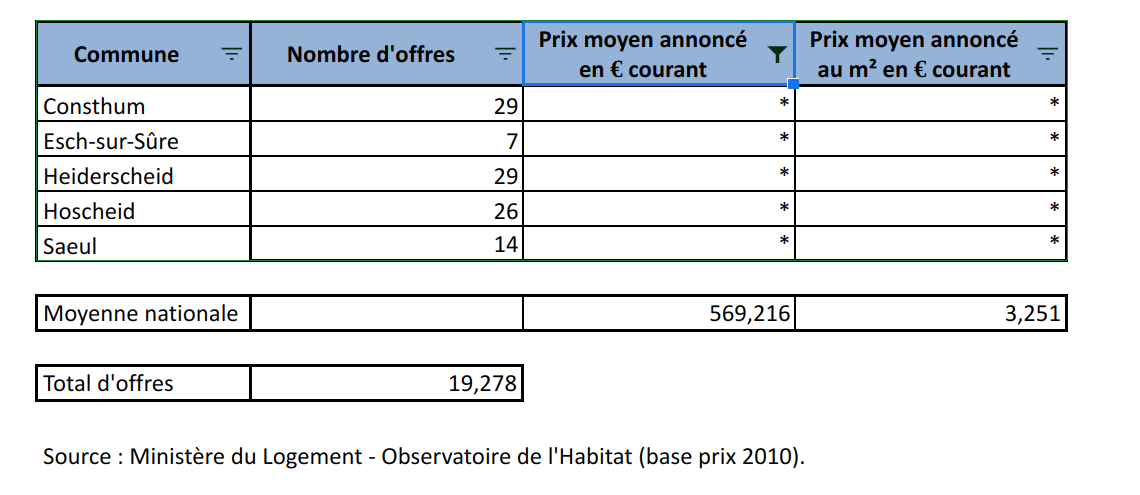
\includegraphics[width=3.8in,height=\textheight]{images/obs_hab_xlsx_missing.png}

}

\caption{Always look at your data.}

\end{figure}

So it turns out that there are some rows that we need to remove. We can
start by removing rows where \texttt{locality} is missing. Then we have
a row where \texttt{locality} is equal to ``Total d'offres''. This is
simply the total of every offer from every commune. We could keep that
in a separate data frame, or even remove it. The very last row states
the source of the data and we can also remove it. Finally, in the
screenshot above, we see another row that we don't see in our filtered
data frame: one where \texttt{n\_offers} is missing. This row gives the
national average for columns \texttt{average\_prince\_nominal\_euros}
and \texttt{average\_price\_m2\_nominal\_euros}. What we are going to do
is create two datasets: one with data on communes, and the other on
national prices. Let's first remove the rows stating the sources:

\begin{Shaded}
\begin{Highlighting}[]
\NormalTok{raw\_data }\OtherTok{\textless{}{-}}\NormalTok{ raw\_data }\SpecialCharTok{|\textgreater{}}
  \FunctionTok{filter}\NormalTok{(}\SpecialCharTok{!}\FunctionTok{grepl}\NormalTok{(}\StringTok{"Source"}\NormalTok{, locality))}
\end{Highlighting}
\end{Shaded}

Let's now only keep the communes in our data:

\begin{Shaded}
\begin{Highlighting}[]
\NormalTok{commune\_level\_data }\OtherTok{\textless{}{-}}\NormalTok{ raw\_data }\SpecialCharTok{|\textgreater{}}
    \FunctionTok{filter}\NormalTok{(}\SpecialCharTok{!}\FunctionTok{grepl}\NormalTok{(}\StringTok{"nationale|offres"}\NormalTok{, locality),}
           \SpecialCharTok{!}\FunctionTok{is.na}\NormalTok{(locality))}
\end{Highlighting}
\end{Shaded}

And let's create a dataset with the national data as well:

\begin{Shaded}
\begin{Highlighting}[]
\NormalTok{country\_level }\OtherTok{\textless{}{-}}\NormalTok{ raw\_data }\SpecialCharTok{|\textgreater{}}
  \FunctionTok{filter}\NormalTok{(}\FunctionTok{grepl}\NormalTok{(}\StringTok{"nationale"}\NormalTok{, locality)) }\SpecialCharTok{|\textgreater{}}
  \FunctionTok{select}\NormalTok{(}\SpecialCharTok{{-}}\NormalTok{n\_offers)}

\NormalTok{offers\_country }\OtherTok{\textless{}{-}}\NormalTok{ raw\_data }\SpecialCharTok{|\textgreater{}}
  \FunctionTok{filter}\NormalTok{(}\FunctionTok{grepl}\NormalTok{(}\StringTok{"Total d.offres"}\NormalTok{, locality)) }\SpecialCharTok{|\textgreater{}}
  \FunctionTok{select}\NormalTok{(year, n\_offers)}

\NormalTok{country\_level\_data }\OtherTok{\textless{}{-}} \FunctionTok{full\_join}\NormalTok{(country\_level, offers\_country) }\SpecialCharTok{|\textgreater{}}
  \FunctionTok{select}\NormalTok{(year, locality, n\_offers, }\FunctionTok{everything}\NormalTok{()) }\SpecialCharTok{|\textgreater{}}
  \FunctionTok{mutate}\NormalTok{(}\AttributeTok{locality =} \StringTok{"Grand{-}Duchy of Luxembourg"}\NormalTok{)}
\end{Highlighting}
\end{Shaded}

\begin{verbatim}
Joining with `by = join_by(year)`
\end{verbatim}

Now the data looks clean, and we can start the actual analysis\ldots{}
or can we? Before proceeding, it would be nice to make sure that we got
every commune in there. For this, we need a list of communes from
Luxembourg.
\href{https://en.wikipedia.org/wiki/List_of_communes_of_Luxembourg}{Thankfully,
Wikipedia has such a list}\footnote{https://w.wiki/6nPu}.

An issue with scraping tables off the web is that they might change in
the future. It is therefore a good idea to save the page by right
clicking on it and then selecting save as, and then re-hosting it. I use
Github pages to re-host the Wikipedia page above
\href{https://b-rodrigues.github.io/list_communes/}{here}\footnote{https://is.gd/lux\_communes}.
I now have full control of this page, and won't get any bad surprises if
someone decides to eventually update it. Instead of re-hosting it, you
could simply save it as any other file of your project.

So let's scrape and save this list:

\begin{Shaded}
\begin{Highlighting}[]
\NormalTok{current\_communes }\OtherTok{\textless{}{-}} \StringTok{"https://is.gd/lux\_communes"} \SpecialCharTok{|\textgreater{}}
\NormalTok{  rvest}\SpecialCharTok{::}\FunctionTok{read\_html}\NormalTok{() }\SpecialCharTok{|\textgreater{}}
\NormalTok{  rvest}\SpecialCharTok{::}\FunctionTok{html\_table}\NormalTok{() }\SpecialCharTok{|\textgreater{}}
\NormalTok{  purrr}\SpecialCharTok{::}\FunctionTok{pluck}\NormalTok{(}\DecValTok{2}\NormalTok{) }\SpecialCharTok{|\textgreater{}}
\NormalTok{  janitor}\SpecialCharTok{::}\FunctionTok{clean\_names}\NormalTok{() }\SpecialCharTok{|\textgreater{}}
\NormalTok{  dplyr}\SpecialCharTok{::}\FunctionTok{filter}\NormalTok{(name\_2 }\SpecialCharTok{!=} \StringTok{"Name"}\NormalTok{) }\SpecialCharTok{|\textgreater{}}
\NormalTok{  dplyr}\SpecialCharTok{::}\FunctionTok{rename}\NormalTok{(}\AttributeTok{commune =}\NormalTok{ name\_2) }\SpecialCharTok{|\textgreater{}}
\NormalTok{  dplyr}\SpecialCharTok{::}\FunctionTok{mutate}\NormalTok{(}\AttributeTok{commune =}\NormalTok{ stringr}\SpecialCharTok{::}\FunctionTok{str\_remove}\NormalTok{(commune, }\StringTok{" .$"}\NormalTok{))}
\end{Highlighting}
\end{Shaded}

We scrape the table from the re-hosted Wikipedia page using
\texttt{\{rvest\}}. \texttt{rvest::html\_table()} returns a list of
tables from the Wikipedia table, and then we use \texttt{purrr::pluck()}
to keep the second table from the website, which is what we need (I made
the calls to the packages explicit, because you might not be familiar
with these packages). \texttt{janitor::clean\_names()} transforms column
names written for human eyes into machine-friendly names (for example
\texttt{Growth\ rate\ in\ \%} would be transformed to
\texttt{growth\_rate\_in\_percent}) and then I use the
\texttt{\{dplyr\}} package for some further cleaning and renaming; the
very last step removes a dagger symbol next to certain communes names,
in other words it turns ``Commune †'' into ``Commune''.

Let's see if we have all the communes in our data:

\begin{Shaded}
\begin{Highlighting}[]
\FunctionTok{setdiff}\NormalTok{(}\FunctionTok{unique}\NormalTok{(commune\_level\_data}\SpecialCharTok{$}\NormalTok{locality),}
\NormalTok{        current\_communes}\SpecialCharTok{$}\NormalTok{commune)}
\end{Highlighting}
\end{Shaded}

\begin{verbatim}
 [1] "Bascharage"          "Boevange-sur-Attert" "Burmerange"         
 [4] "Clémency"            "Consthum"            "Ermsdorf"           
 [7] "Erpeldange"          "Eschweiler"          "Heiderscheid"       
[10] "Heinerscheid"        "Hobscheid"           "Hoscheid"           
[13] "Hosingen"            "Luxembourg"          "Medernach"          
[16] "Mompach"             "Munshausen"          "Neunhausen"         
[19] "Rosport"             "Septfontaines"       "Tuntange"           
[22] "Wellenstein"         "Kaerjeng"           
\end{verbatim}

We see many communes that are in our \texttt{commune\_level\_data}, but
not in \texttt{current\_communes}. There's one obvious reason:
differences in spelling, for example, ``Kaerjeng'' in our data, but
``Käerjeng'' in the table from Wikipedia. But there's also a less
obvious reason; since 2010, several communes have merged into new ones.
So there are communes that are in our data in 2010 and 2011, but
disappear from 2012 onwards. So we need to do several things: first, get
a list of all existing communes from 2010 onwards, and then, harmonise
spelling. Here again, we can use a list from Wikipedia, and here again,
I decide to re-host it on Github pages to avoid problems in the future:

\begin{Shaded}
\begin{Highlighting}[]
\NormalTok{former\_communes }\OtherTok{\textless{}{-}} \StringTok{"https://is.gd/lux\_former\_communes"} \SpecialCharTok{|\textgreater{}}
\NormalTok{  rvest}\SpecialCharTok{::}\FunctionTok{read\_html}\NormalTok{() }\SpecialCharTok{|\textgreater{}}
\NormalTok{  rvest}\SpecialCharTok{::}\FunctionTok{html\_table}\NormalTok{() }\SpecialCharTok{|\textgreater{}}
\NormalTok{  purrr}\SpecialCharTok{::}\FunctionTok{pluck}\NormalTok{(}\DecValTok{3}\NormalTok{) }\SpecialCharTok{|\textgreater{}}
\NormalTok{  janitor}\SpecialCharTok{::}\FunctionTok{clean\_names}\NormalTok{() }\SpecialCharTok{|\textgreater{}}
\NormalTok{  dplyr}\SpecialCharTok{::}\FunctionTok{filter}\NormalTok{(year\_dissolved }\SpecialCharTok{\textgreater{}} \DecValTok{2009}\NormalTok{)}

\NormalTok{former\_communes}
\end{Highlighting}
\end{Shaded}

\begin{verbatim}
# A tibble: 20 x 3
   name                year_dissolved reason                         
   <chr>                        <int> <chr>                          
 1 Bascharage                    2011 merged to form Käerjeng        
 2 Boevange-sur-Attert           2018 merged to form Helperknapp     
 3 Burmerange                    2011 merged into Schengen           
 4 Clemency                      2011 merged to form Käerjeng        
 5 Consthum                      2011 merged to form Parc Hosingen   
 6 Ermsdorf                      2011 merged to form Vallée de l'Ernz
 7 Eschweiler                    2015 merged into Wiltz              
 8 Heiderscheid                  2011 merged into Esch-sur-Sûre      
 9 Heinerscheid                  2011 merged into Clervaux           
10 Hobscheid                     2018 merged to form Habscht         
11 Hoscheid                      2011 merged to form Parc Hosingen   
12 Hosingen                      2011 merged to form Parc Hosingen   
13 Mompach                       2018 merged to form Rosport-Mompach 
14 Medernach                     2011 merged to form Vallée de l'Ernz
15 Munshausen                    2011 merged into Clervaux           
16 Neunhausen                    2011 merged into Esch-sur-Sûre      
17 Rosport                       2018 merged to form Rosport-Mompach 
18 Septfontaines                 2018 merged to form Habscht         
19 Tuntange                      2018 merged to form Helperknapp     
20 Wellenstein                   2011 merged into Schengen           
\end{verbatim}

As you can see, since 2010 many communes have merged to form new ones.
We can now combine the list of current and former communes, as well as
harmonise their names:

\begin{Shaded}
\begin{Highlighting}[]
\NormalTok{communes }\OtherTok{\textless{}{-}} \FunctionTok{unique}\NormalTok{(}\FunctionTok{c}\NormalTok{(former\_communes}\SpecialCharTok{$}\NormalTok{name,}
\NormalTok{                     current\_communes}\SpecialCharTok{$}\NormalTok{commune))}
\CommentTok{\# we need to rename some communes}

\CommentTok{\# Different spelling of these communes between wikipedia and the data}

\NormalTok{communes[}\FunctionTok{which}\NormalTok{(communes }\SpecialCharTok{==} \StringTok{"Clemency"}\NormalTok{)] }\OtherTok{\textless{}{-}} \StringTok{"Clémency"}
\NormalTok{communes[}\FunctionTok{which}\NormalTok{(communes }\SpecialCharTok{==} \StringTok{"Redange"}\NormalTok{)] }\OtherTok{\textless{}{-}} \StringTok{"Redange{-}sur{-}Attert"}
\NormalTok{communes[}\FunctionTok{which}\NormalTok{(communes }\SpecialCharTok{==} \StringTok{"Erpeldange{-}sur{-}Sûre"}\NormalTok{)] }\OtherTok{\textless{}{-}} \StringTok{"Erpeldange"}
\NormalTok{communes[}\FunctionTok{which}\NormalTok{(communes }\SpecialCharTok{==} \StringTok{"Luxembourg City"}\NormalTok{)] }\OtherTok{\textless{}{-}} \StringTok{"Luxembourg"}
\NormalTok{communes[}\FunctionTok{which}\NormalTok{(communes }\SpecialCharTok{==} \StringTok{"Käerjeng"}\NormalTok{)] }\OtherTok{\textless{}{-}} \StringTok{"Kaerjeng"}
\NormalTok{communes[}\FunctionTok{which}\NormalTok{(communes }\SpecialCharTok{==} \StringTok{"Petange"}\NormalTok{)] }\OtherTok{\textless{}{-}} \StringTok{"Pétange"}
\end{Highlighting}
\end{Shaded}

Let's run our test again:

\begin{Shaded}
\begin{Highlighting}[]
\FunctionTok{setdiff}\NormalTok{(}\FunctionTok{unique}\NormalTok{(commune\_level\_data}\SpecialCharTok{$}\NormalTok{locality),}
\NormalTok{        communes)}
\end{Highlighting}
\end{Shaded}

\begin{verbatim}
character(0)
\end{verbatim}

Great! When we compare the communes that are in our data with every
commune that has existed since 2010, we don't have any commune that is
unaccounted for. So are we done with cleaning the data? Yes, we can now
start with analysing the data. Take a look
\href{https://raw.githubusercontent.com/b-rodrigues/rap4all/master/scripts/save_data.R}{here}\footnote{https://is.gd/7PhUjd}
to see the finalised script. Also read some of the comments that I've
added. This is a typical R script, and at first glance, one might wonder
what is wrong with it. Actually, not much, but the problem if you leave
this script as it is, is that it is very likely that we will have
problems rerunning it in the future. As it turns out, this script is not
reproducible. But we will discuss this in much more detail later on. For
now, let's analyse our cleaned data.

\hypertarget{project-analysis}{%
\subsection{Project Analysis}\label{project-analysis}}

We are now going to analyse the data.



\end{document}
